\documentclass[a4paper]{article}
\usepackage[utf8]{inputenc}
\usepackage[russian]{babel}
\usepackage{listings}
\usepackage[a4paper]{geometry}
\usepackage{indentfirst}
\usepackage{graphicx}
\usepackage{caption}
\usepackage{float}

\begin{document}

\title{Лабораторная работа 2 по курсу <<Нелинейная динамика и её приложения>>. \\Отчёт.}
\author{Владислав Соврасов\\ 381503м4}
\date{}
\maketitle

\section{Построение бифуркационной диаграммы}
Рассматривается система авторепрессора с задержкой:
\begin{displaymath}
  \dot x = \frac{\alpha}{1+x^N(t-\tau)} - x
\end{displaymath}
Для этой системы необходимо построить бифуркационную диаграмму на плоскости
\((\alpha,\tau)\). Количество и положение состояний равновесия авторепрессора с
задержкой не отличаются от системы без задержки. Комбинация параметров влияет
на устойчивость единственного состояния равновесия.

Бифуркационное условие определяется уравнениями:
\begin{displaymath}
	\left\{
  \begin{array}{lr}
    x_0^{N+1}+x_0-\alpha = 0 \\
    \omega^2=N^2(1-\frac{x_0}{\alpha})^2-1 \\
    cos(\omega \tau)=-\frac{1}{N(1-\frac{x_0}{\alpha})}
  \end{array}
\right.
\end{displaymath}
Задав значение \(\alpha\) и решив первое уравнение, можно найти значение \(\omega\),
подставив во второе уравнение \(x_0\). Затем \(\tau\) находится из третьего
уравнения по явной формуле \(\tau = \frac{1}{\omega}arccos(-\frac{1}{N(1-\frac{x_0}{\alpha})})\).

На рис. \ref{fig:diagram} представленная найденная описанным способом бифуркационная
кривая при \(N=2,4,6\). Если задать точку \((\alpha,\tau)\) выше кривой, то система
будет переходить в режим автоколебаний. Если точка ниже кривой, то авторепрессор с
задержкой имеет одно устойчивое состояние равновесия.
\begin{figure}[H]
	\center
  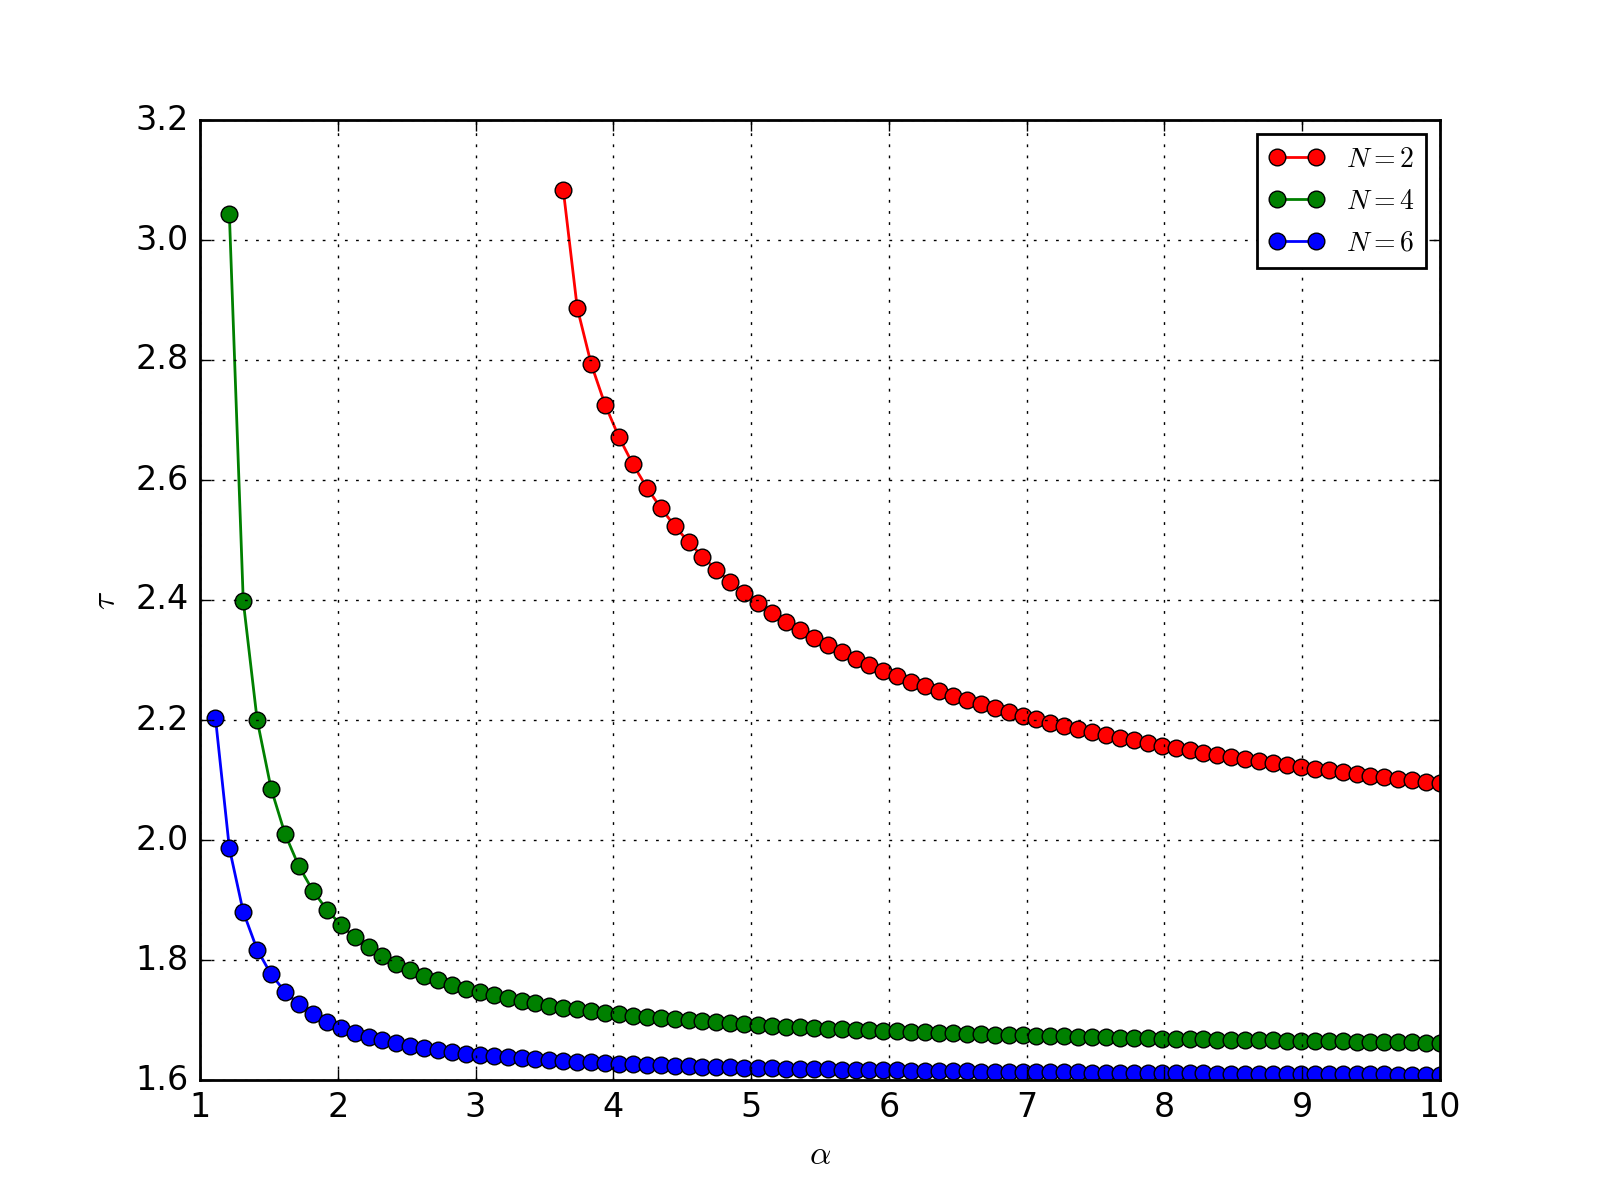
\includegraphics[width=0.75\textwidth]{../pictures/lab2_diagram.png}
  \caption{Бифуркационная диаграмма системы при различных значениях \(N\)}
  \label{fig:diagram}
\end{figure}


\section{Исходный код}

\lstinputlisting[language=Python, numbers=left]{../scripts/lab2.py}

\end{document}
